\subsection{Model}\label{sec:cloud:crowdsourcing:model}

In our model, schematically depicted in \reffig{fig:sec:cloud:crowdsourcing:model:model}, we consider a crowdsourcing  platform employing \(\numberOfWorkers\) workers.
The time between two campaigns being submitted is given by the random variable \(\campaignIAT\)
Each campaign consists of a number of tasks, distributed according to the random variable \(\campaignSize\).
We assume that each task is then completed by one of the \(\numberOfWorkers\) workers in order of arrival.
The time required for completion is given by the random variable \(\taskDuration\).

\begin{figure}
  \centering
  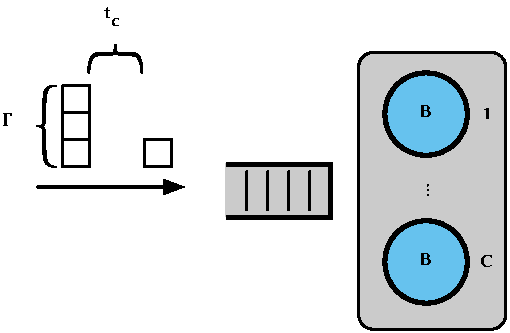
\includegraphics{cloud/crowdsourcing/model/figures/model}
  \caption{Crowdsourcing Platform Model}
  \label{fig:sec:cloud:crowdsourcing:model:model}
\end{figure}

From this model we derive two metrics in order to evaluate the performance of the crowdsourcing platform.
First, we consider the utilization \(\workerUtilization\) for all workers.
This can be interpreted as a measure for workers about how much they can earn on the platform and should be maximized in order to keep current workers and attract new ones. 
Furthermore, we seek to obtain the mean task pre-processing delay \(\preTaskProcessingDelay\), i.e., the time occurring before a worker begins to work on a task.
This measure is relevant for the employer and should be minimized.
We use the \(\preTaskProcessingDelay\) instead of the average completion time of the campaigns, as the completion time also depends on the task length, which is under control of the employer and not the platform operator.

In this section we first introduce an analytical model, which will be used to validate the simulation model discussed thereafter.
Finally, a comparative validation of the analytical and simulative model is then performed.

\subsubsection*{Analytical Consideration}

First, in order to provide exact results, we consider the crowdsourcing platform as a \(M^{[\campaignSize]}/M/\numberOfWorkers-\infty\) model.
Here, we assume both the campaign inter-arrival time \(\campaignIAT\) as well as the time to complete a task \(\taskDuration\) to be exponentially distributed with mean \(E[\campaignIAT] = \frac{1}{\lambda}\) and \(E[B] = \nicefrac{1}{\mu}\), due to the large number of employers submitting tasks and the large number of workers completing them.
Furthermore, we model the number of tasks per campaign \(\campaignSize\) using a geometric distribution with mean \(E[\campaignSize] = \nicefrac{1}{p}\).

State probabilities\cite{Kleinrock1975} can be obtained by solving the state equations, yielding
\[
x(i + 1) = x(i) \frac{\lambda + \mu \min(i, c)}{\mu \min(i + 1, c)} - \sum_{k=0}^{i-1} x(k) \lambda \theta(i - k)
\]
for \(i \geq 0\) tasks unserviced in the platform.
The state probability for \(x(i+1)\) only depends on the state probabilities for \(x(k)\) for \(k \leq i\) lending itself to an iterative numerical computation.
Note that \(x(0)\) cannot be computed in such a manner and has to be obtained using the normalizing equation \(1 = \sum_{i=0}^{\infty} x(i)\).

Thus, we first calculate \(x(1)\) as a multiple of \(x(0)\) that is \(x(1) = \zeta(1) x(0)\).
Then, we compute each \(x(i)\) depending on the previously computed values for \(x(j), j \leq i\) and thus obtain expressions \(x(i) = \zeta(i) x(0)\).  
Once a sufficient number \(\kappa\) of state probabilities have been computed, the normalizing property is applied, and \(x(0)\) is computed as
\[
	x(0) = \left(1 + \sum_{i = 1}^\kappa \zeta(i)\right)^{-1}.
\]
Finally, we can calculate the actual state probabilities as \(x(i) = \zeta(i) x(0)\) for all \(0 < i \leq \kappa\).

Based on these state probabilities, we obtain the mean worker utilization as
\[
\workerUtilization = \sum_{i=0}^{\kappa} \min(i, c) x(i) = \frac{\lambda E[\campaignSize]}{c\mu}. 
\]

Next, we obtain the mean queue length \(\Omega\) of the system as
\[
	\Omega = \sum_{i = c}^\kappa (i - c) x(i).
\]
Now, we consider the mean task pre-processing delay and with Little's theorem applied to the systems queue, we get
\[\lambda E[\campaignSize] \preTaskProcessingDelay = \Omega.\]

We solve for task the pre-processing delay \preTaskProcessingDelay~and obtain
\[\preTaskProcessingDelay = \frac{\Omega}{\lambda E[\campaignSize]}.\]

\subsubsection*{Simulation}

In order to allow for a larger variety of campaign inter-arrival time distributions, we implement a discrete event simulation using the OMNet++ simulation framework\footnote{\url{http://www.omnetpp.org/}, Accessed Jul 2015}.
We augment the framework with support for bulk arrivals and support of empiric distributions taken from measurements described in \refsec{sec:cloud:crowdsourcing:measurements}.
Similar, to the queueing model introduced in this section, we consider campaign inter-arrivals according to a distribution \(\campaignIAT\) and a campaign size of \(\campaignSize\) tasks.
Task length is given by a distribution \(\taskDuration\) and tasks are stored in an unbounded queue before being sent to service to the available workers \(\numberOfWorkers\).
During simulation, we record the mean worker utilization \(\workerUtilization\) as well as the mean task pre-processing delay \(\preTaskProcessingDelay\).

\subsubsection*{Validation}

In this section, we validate the simulative model by comparing the metrics \(\workerUtilization\) and \(\preTaskProcessingDelay\) for a representative parameter set with those obtained from the analytic model.
We consider exponential campaign inter-arrival times with a campaign rate of \SI{4}{\per\hour}  campaigns per hour, and a campaign size \campaignSize geometrically distributed with a mean of \(100\) tasks per campaign.
For the task duration \taskDuration we consider a set of suitable values, to accommodate for different task types, between \SIrange{60}{300}{\minute} per task.
In both simulation and analytical model, we consider between $5$ and $50$ workers.
